\chapter{The standard model}

\section{Introduction}
Sample text sample text sample text. Sample text sample text sample text.
Sample text sample text sample text. Sample text sample text sample text.
Sample text sample text sample text. Sample text sample text sample text.

The elementary particles defined in the standard model are demonstrated in Fig~\ref{fig:c1smparticletable}.
% Standard model particle table
\begin{figure}[htbp]
  \begin{center}
    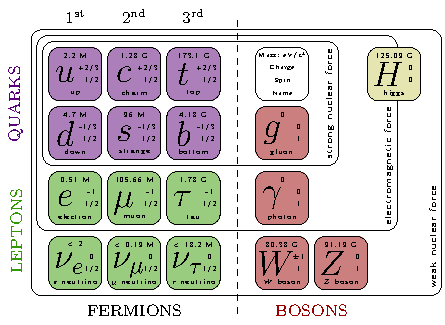
\includegraphics[width=0.8\textwidth]{chapters/c1/figures/sm-particle-table.pdf}
  \end{center}
  \caption{Particles of the Standard Model of particle physics}
  \label{fig:c1smparticletable}
\end{figure}

The standard model Lagrangian is shown in Eq~\ref{eq:c1sml}:
% Standard model equation
\begin{equation}
  \begin{alignedat}{2}
  L = & -\frac{1}{4}B_{\mu\nu}B^{\mu\nu} - \frac{1}{8}tr(F_{\mu\nu}F^{\mu\nu}) - \frac{1}{2}tr(G_{\mu\nu}G^{\mu\nu}), (Gauge \, terms) \\
      & +\begin{pmatrix} \bar{\nu}_{L} & \bar{e}_{L} \end{pmatrix}\bar{\sigma}^{\mu}iD_{\mu}\begin{pmatrix} \nu_{L} \\ e_{L} \end{pmatrix} + \bar{e}_{R}\sigma^{\mu}iD_{\mu}e_{R} + \bar{\nu}_{R}\sigma^{\mu}iD_{\mu}\nu_{R}, (Lepton \, dynamical \, terms) \\
      & -\frac{\sqrt{2}}{\upsilon}[\begin{pmatrix} \bar{\nu}_{L} & \bar{e}_{L} \end{pmatrix}\phi M^{e}e_{R} + \bar{e}_{R}\bar{M}^{e}\bar{\phi}\begin{pmatrix} \nu_{L} \\ e_{L} \end{pmatrix}], (Electron, muon, Tau \, mass \, terms) \\
      & -\frac{\sqrt{2}}{\upsilon}[\begin{pmatrix} -\bar{e}_{L} & \bar{\nu}_{L} \end{pmatrix}\phi^{*} M^{\nu}\nu_{R} + \bar{\nu}_{R}\bar{M}^{\nu}\phi^{T}\begin{pmatrix} -e_{L} \\ \nu_{L} \end{pmatrix}], (Neutrino \, mass \, terms) \\
      & +\begin{pmatrix} \bar{u}_{L} & \bar{d}_{L} \end{pmatrix}\bar{\sigma}^{\mu}iD_{\mu}\begin{pmatrix} u_{L} \\ d_{L} \end{pmatrix} + \bar{u}_{R}\sigma^{\mu}iD_{\mu}u_{R} + \bar{d}_{R}\sigma^{\mu}iD_{\mu}d_{R}, (quark \, dynamical \, terms) \\
      & -\frac{\sqrt{2}}{\upsilon}[\begin{pmatrix} \bar{u}_{L} & \bar{d}_{L} \end{pmatrix}\phi M^{d}d_{R} + \bar{d}_{R}\bar{M}^{d}\bar{\phi}\begin{pmatrix} u_{L} \\ d_{L} \end{pmatrix}], (Down, strange, bottom \, mass \, terms) \\
      & -\frac{\sqrt{2}}{\upsilon}[\begin{pmatrix} -\bar{d}_{L} & \bar{u}_{L} \end{pmatrix}\phi^{*} M^{u}u_{R} + \bar{u}_{R}\bar{M}^{u}\phi^{T}\begin{pmatrix} -d_{L} \\ u_{L} \end{pmatrix}], (Up, charm, top \, mass \, terms) \\
      & +\bar{D_{\mu}\phi}D^{\mu}\phi - m_{h}^{2}[\bar{\phi}\phi-\upsilon^{2}/2]^{2}/2\upsilon^{2}, (Higgs \, dynamical \, and \, mass \, terms)
  \label{eq:c1sml}
  \end{alignedat}
\end{equation}

The definition of derivative operators in the Eq~\ref{eq:c1sml} are:
\begin{equation}
  \begin{aligned}
  D_{\mu}\begin{pmatrix} \nu_{L} \\ e_{L} \end{pmatrix} = [\partial_{\mu}-\frac{ig_{1}}{2}B_{\mu}+\frac{ig_{2}}{2}W_{\mu}]\begin{pmatrix} \nu_{L} \\ e_{L} \end{pmatrix} \\
  D_{\mu}\nu_{R} = \partial_{\mu}\nu_{R},\quad D_{\mu}e_{R} = [\partial_{\mu}-ig_{1}B_{\mu}]e_{R}
  \end{aligned}
  \label{eq:c1smldl}
\end{equation}

\begin{equation}
  \begin{aligned}
  D_{\mu}\begin{pmatrix} u_{L} \\ d_{L} \end{pmatrix} = [\partial_{\mu}+\frac{ig_{1}}{6}B_{\mu}+\frac{ig_{2}}{2}W_{\mu}+igG_{\mu}]\begin{pmatrix} u_{L} \\ d_{L} \end{pmatrix} \\
  D_{\mu}u_{R} = [\partial_{\mu}+\frac{i2g_{1}}{3}B_{\mu}+igG_{\mu}]u_{R},\quad D_{\mu}d_{R} = [\partial_{\mu}-\frac{ig_{1}}{3}B_{\mu}+igG_{\mu}]d_{R}
  \end{aligned}
  \label{eq:c1smldq}
\end{equation}

\begin{equation}
  \begin{aligned}
  D_{\mu}\phi = [\partial_{\mu}+\frac{ig_{1}}{2}B_{\mu}+\frac{ig_{2}}{2}W_{\mu}]\phi
  \end{aligned}
  \label{eq:c1smldh}
\end{equation}

\section{Challenges}
Sample text sample text sample text. Sample text sample text sample text.
Sample text sample text sample text. Sample text sample text sample text.
Sample text sample text sample text. Sample text sample text sample text.
